\newpage
\section{Angabe}
    Implementieren Sie Quicksort (https://de.wikipedia.org/wiki/Quicksort) für arrays mit integern. Testen und Messen sie die Zeiten mit 10, 100, 1000, 10000, 100000 Elementen.\\

    \noindent Bonus Aufgabe: Messreihe und Vergleich mit Bubblesort, messen gegen qsort(3) aus der C Bibliothek.

    \begin{lstlisting}[language=C, style=CStyle, caption=Gegebener-Code, captionpos=b, label=init-CLOCK]
#include <assert.h>
#include <stdio.h>
#include <stdlib.h>
#include <time.h>

void qs(int *a, int us, int os)
{
	// TODO
}

// creates a array of size size and fills it with random ints in range 0 to max_int
int *create_array(int size, int max_int)
{
	int *b = (int*)malloc(size * sizeof(int));

	for (int i=0; i<size; i++) {
		b[i] = rand() % max_int;
	}

	return b;
}

#define MY_SIZE 32

int main(int argc, char **argv)
{
	// create random ints based in current time
	srand(time(NULL));

        int *a = create_array(MY_SIZE, 100);

	qs(a, 0, MY_SIZE);

	int old = -1;
	for (int i=0; i<MY_SIZE; ++i)      {
		if (old != -1) assert(old <= a[i]);
		printf("%d ", a[i]);
		old = a[i];
	}
	printf("\n");
}
        \end{lstlisting}

\section{Lösung}
    Die Lösung für den QSort Algorithmus wurde mithilfe des Pseudocodes des wikipedia Artikels \url{https://de.wikipedia.org/wiki/Quicksort} erstellt.\\
    Bublesort wurde aus einem alten Projekt herausgenommen.\\   
    \textbf{Der Code mit Makefile ist in dem extra Zip Ordner oder auf GitHub zu finden: \url{https://github.com/FabioPlunser/FSST_Lezuo/tree/main/Programme/Sortieren}}
\section{Ergebnisse}
    Der Plot hat die Größe des Arrays auf der X-Achse und die Zeitdauer auf der Y-Achse. 

    \begin{figure}[!htb]
        \centering
        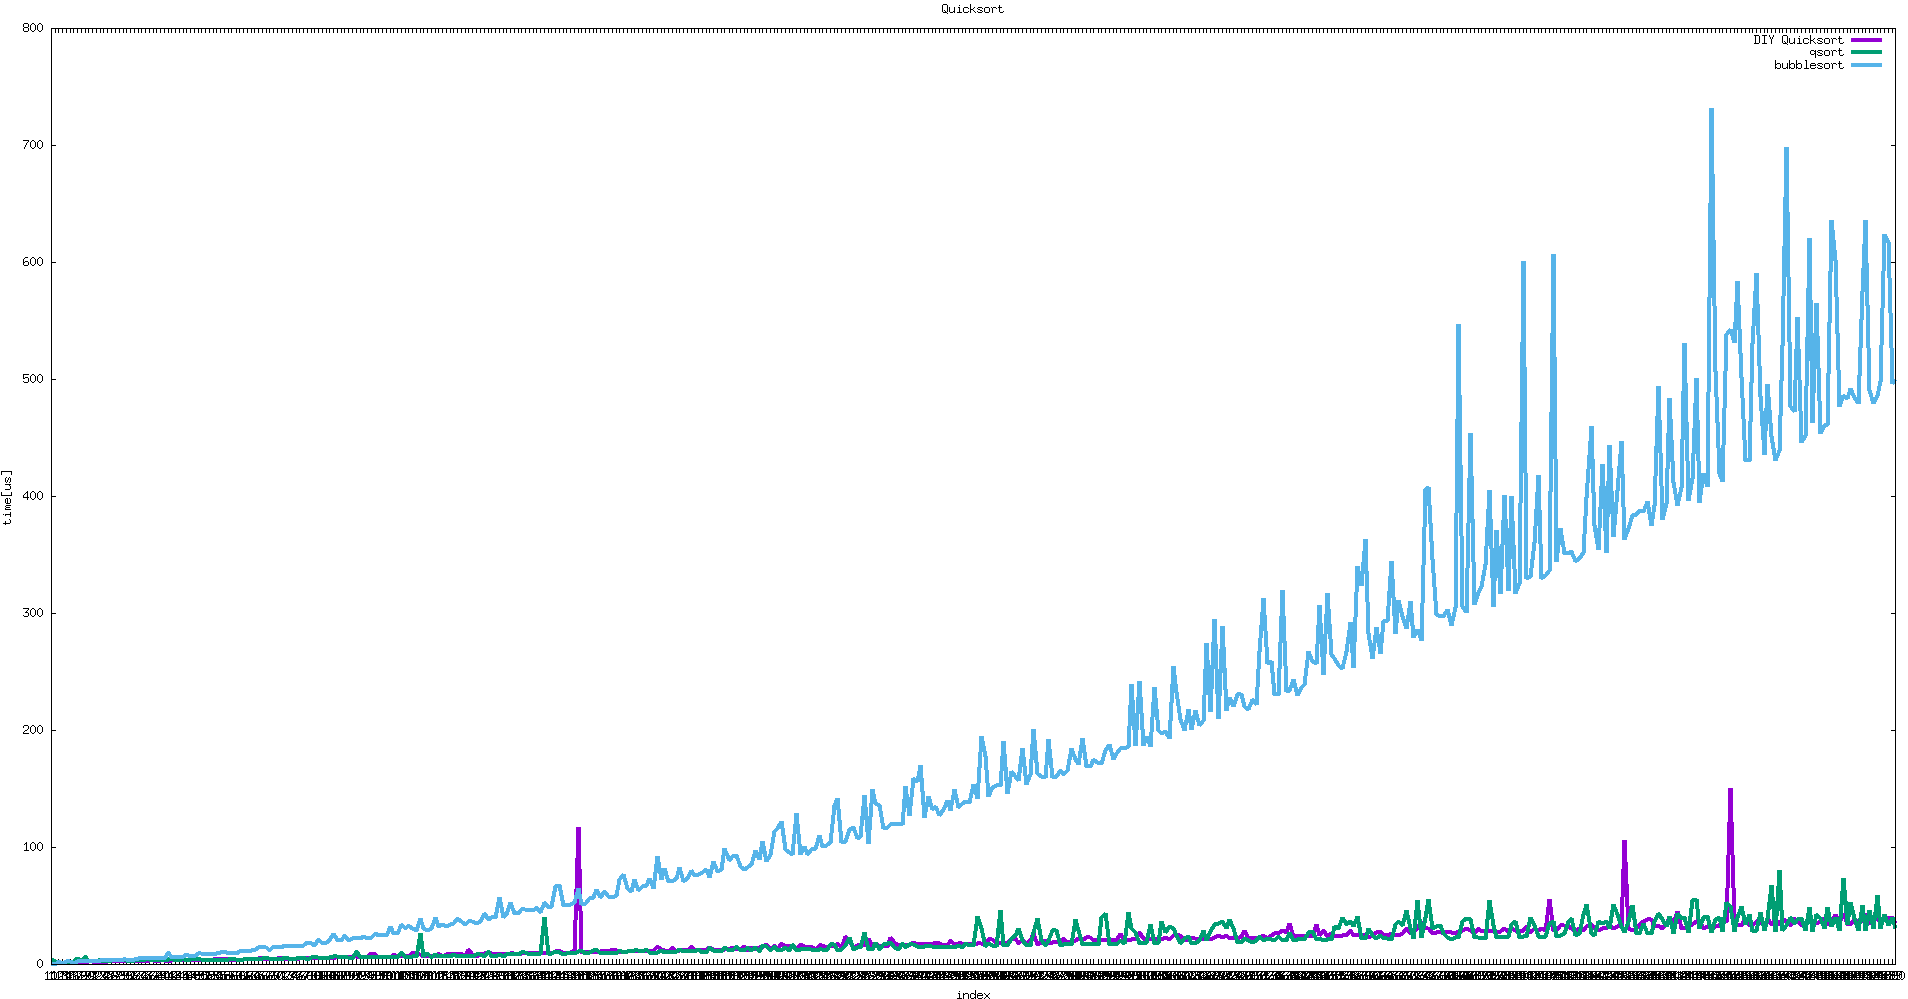
\includegraphics[width=\linewidth]{Plot-Ergebnis-max-1000.png}
        \caption{Plot-Ergebnis-max-1000}
        \label{caption:Plot-Ergebnis-max-1000}
    \end{figure}

    \noindent Man sieht, dass Bubblesort bei zunehmender Größe des Arrays immer länger Zeit benötigt, wo die anderen Algorithmen immer ungefähr gleich lang brauchen. 